\documentclass[aspectratio=169,11pt]{beamer}

\usetheme{Madrid}
\usecolortheme{beaver}

% Custom Colors
\definecolor{primaryblue}{RGB}{24, 76, 120}
\definecolor{accentteal}{RGB}{20, 110, 120}
\definecolor{darkslate}{RGB}{35, 45, 55}

\setbeamercolor{palette primary}{bg=primaryblue,fg=white}
\setbeamercolor{palette secondary}{bg=accentteal,fg=white}
\setbeamercolor{palette tertiary}{bg=darkslate,fg=white}
\setbeamercolor{titlelike}{parent=palette primary,fg=primaryblue}
\setbeamercolor{structure}{fg=primaryblue}
\setbeamercolor{block title}{bg=primaryblue!15,fg=primaryblue}
\setbeamercolor{block body}{bg=gray!8,fg=black}

\setbeamertemplate{navigation symbols}{}

% Clean footline without B.Tech
\setbeamertemplate{footline}{
  \leavevmode%
  \hbox{%
  \begin{beamercolorbox}[wd=.333333\paperwidth,ht=2.25ex,dp=1ex,left]{author in head/foot}%
    \hspace*{2ex}\usebeamerfont{author in head/foot}\textbf{Aarti Kushwaha}
  \end{beamercolorbox}%
  \begin{beamercolorbox}[wd=.333333\paperwidth,ht=2.25ex,dp=1ex,center]{title in head/foot}%
    \usebeamerfont{title in head/foot}File Compression System
  \end{beamercolorbox}%
  \begin{beamercolorbox}[wd=.333333\paperwidth,ht=2.25ex,dp=1ex,right]{date in head/foot}%
    \usebeamerfont{date in head/foot}\insertframenumber{} / \inserttotalframenumber\hspace*{2ex}
  \end{beamercolorbox}}%
  \vskip0pt%
}

\usepackage{booktabs}
\usepackage{tabularx}
\usepackage{tikz}
\usetikzlibrary{shapes.geometric,arrows.meta,positioning,calc}

\title[File Compression System]{\textbf{File Compression System Using Huffman Coding}}
\subtitle{Project Proposal Defense Presentation}
\author{\textbf{Aarti Kushwaha}}
\institute{2026}
\date{2026}

\begin{document}

% -----------------------------------------------------------------------------
% SLIDE 1: TITLE SLIDE
% -----------------------------------------------------------------------------
\begin{frame}
    \titlepage
\end{frame}

% -----------------------------------------------------------------------------
% SLIDE 2: INTRODUCTION & BACKGROUND
% -----------------------------------------------------------------------------
\begin{frame}{1. Introduction \& Background Study}
    \begin{block}{Key Background Concepts}
        \begin{itemize}
            \item \textbf{Data Compression}: Minimizes digital storage footprints and network transmission bandwidth across systems.
            \item \textbf{Lossless Guarantee}: Ensures 100\% exact, bit-for-bit file reconstruction without any distortion or loss of data.
            \item \textbf{Shannon \& Huffman Foundation}: Reaches Shannon entropy lower bound $H(X)$ using optimal, greedy prefix binary codes.
        \end{itemize}
    \end{block}
\end{frame}

% -----------------------------------------------------------------------------
% SLIDE 3: PROBLEM STATEMENT & OBJECTIVES
% -----------------------------------------------------------------------------
\begin{frame}{2. Problem Statement \& Objectives}
    \begin{columns}[T]
        \begin{column}{0.48\textwidth}
            \begin{block}{Problem Statement}
                \begin{itemize}
                    \item Raw uncompressed text and log files incur heavy storage and bandwidth costs.
                    \item Existing industrial tools operate as opaque, closed-source ``black boxes''.
                    \item Lack of lightweight tools offering verified byte-for-byte fidelity.
                \end{itemize}
            \end{block}
        \end{column}
        
        \begin{column}{0.48\textwidth}
            \begin{block}{Key Project Objectives}
                \begin{itemize}
                    \item Build a pure, lossless Huffman compression and decompression engine.
                    \item Implement min-heap priority queue for optimal prefix tree synthesis.
                    \item Guarantee 100\% integrity via automated cryptographic SHA-256 checks.
                \end{itemize}
            \end{block}
        \end{column}
    \end{columns}
\end{frame}

% -----------------------------------------------------------------------------
% SLIDE 4: LITERATURE REVIEW
% -----------------------------------------------------------------------------
\begin{frame}{3. Literature Review \& Benchmark}
    \begin{block}{Theoretical Foundation \& Benchmarks}
        \begin{itemize}
            \item \textbf{C. E. Shannon (1948)}: Proved the mathematical limits of data compaction based on source entropy $H(X)$.
            \item \textbf{D. A. Huffman (1952)}: Devised bottom-up greedy binary tree synthesis for minimum-redundancy prefix codes.
            \item \textbf{System Advantage}: Provides transparent, canonical prefix encoding without complex, proprietary black-box layers.
        \end{itemize}
    \end{block}
\end{frame}

% -----------------------------------------------------------------------------
% SLIDE 5: METHODOLOGY & HUFFMAN ALGORITHM
% -----------------------------------------------------------------------------
\begin{frame}{4. Methodology \& Huffman Algorithm Workflow}
    \begin{block}{Three-Phase Compression \& Decompression Pipeline}
        \begin{itemize}
            \item \textbf{Frequency Profiling \& Min-Heap}: Count all 256-byte frequencies and assemble a min-heap priority queue to build the binary tree.
            \item \textbf{Codeword Assignment \& Bit Packing}: Traverse branches (left=`0', right=`1') to generate prefix codes and pack bits into 8-bit bytes with header metadata.
            \item \textbf{Restoration \& Verification}: Parse the header tree, decode the bitstream back to original bytes, and verify SHA-256 hash match.
        \end{itemize}
    \end{block}
\end{frame}

% -----------------------------------------------------------------------------
% SLIDE 6: PROJECT TIMELINE (GANTT CHART DIAGRAM)
% -----------------------------------------------------------------------------
\begin{frame}{5. Project Timeline (4-Month Gantt Chart)}
    \begin{center}
    \resizebox{0.92\textwidth}{!}{
    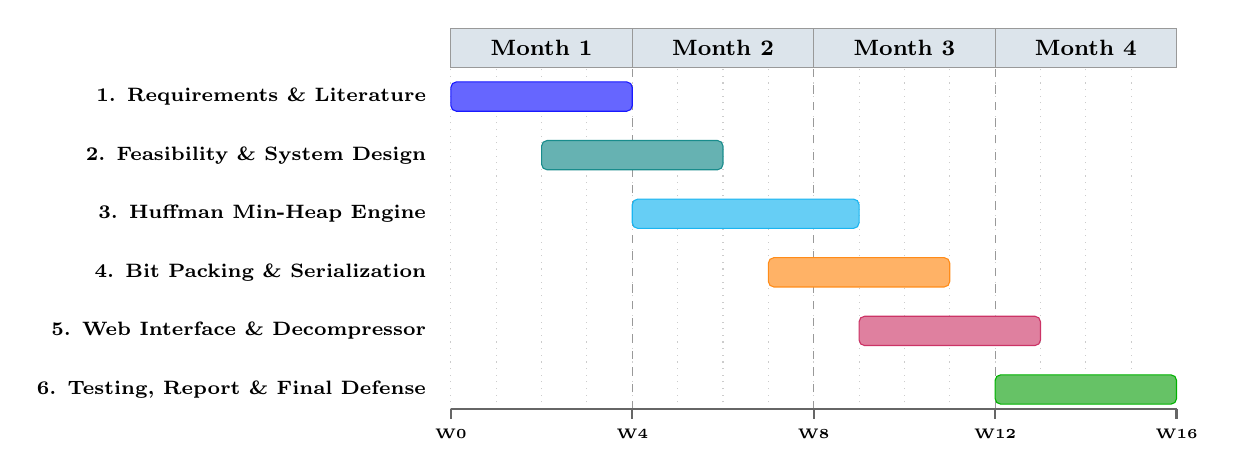
\begin{tikzpicture}[x=0.96cm, y=0.62cm]
        % Month Header Bars
        \draw[fill=primaryblue!15, draw=black!40] (0, 7) rectangle (2.4, 7.8) node[pos=.5, font=\footnotesize\bfseries] {Month 1};
        \draw[fill=primaryblue!15, draw=black!40] (2.4, 7) rectangle (4.8, 7.8) node[pos=.5, font=\footnotesize\bfseries] {Month 2};
        \draw[fill=primaryblue!15, draw=black!40] (4.8, 7) rectangle (7.2, 7.8) node[pos=.5, font=\footnotesize\bfseries] {Month 3};
        \draw[fill=primaryblue!15, draw=black!40] (7.2, 7) rectangle (9.6, 7.8) node[pos=.5, font=\footnotesize\bfseries] {Month 4};
        
        % Grid lines
        \foreach \x in {0, 0.6, ..., 9.6} {
            \draw[dotted, black!20] (\x, 0) -- (\x, 7);
        }
        \foreach \x in {2.4, 4.8, 7.2} {
            \draw[dashed, black!40] (\x, 0) -- (\x, 7);
        }
        
        % Tasks
        \node[anchor=east, font=\scriptsize\bfseries] at (-0.2, 6.4) {1. Requirements \& Literature};
        \draw[fill=blue!60, draw=blue!90, rounded corners=2pt] (0, 6.1) rectangle (2.4, 6.7);
        
        \node[anchor=east, font=\scriptsize\bfseries] at (-0.2, 5.2) {2. Feasibility \& System Design};
        \draw[fill=teal!60, draw=teal!90, rounded corners=2pt] (1.2, 4.9) rectangle (3.6, 5.5);
        
        \node[anchor=east, font=\scriptsize\bfseries] at (-0.2, 4.0) {3. Huffman Min-Heap Engine};
        \draw[fill=cyan!60, draw=cyan!90, rounded corners=2pt] (2.4, 3.7) rectangle (5.4, 4.3);
        
        \node[anchor=east, font=\scriptsize\bfseries] at (-0.2, 2.8) {4. Bit Packing \& Serialization};
        \draw[fill=orange!60, draw=orange!90, rounded corners=2pt] (4.2, 2.5) rectangle (6.6, 3.1);
        
        \node[anchor=east, font=\scriptsize\bfseries] at (-0.2, 1.6) {5. Web Interface \& Decompressor};
        \draw[fill=purple!50, draw=purple!80, rounded corners=2pt] (5.4, 1.3) rectangle (7.8, 1.9);
        
        \node[anchor=east, font=\scriptsize\bfseries] at (-0.2, 0.4) {6. Testing, Report \& Final Defense};
        \draw[fill=green!60!black!60, draw=green!70!black, rounded corners=2pt] (7.2, 0.1) rectangle (9.6, 0.7);
        
        % Axis Base
        \draw[thick, black!60] (0, 0) -- (9.6, 0);
        \foreach \x in {0, 2.4, 4.8, 7.2, 9.6} {
            \draw[thick, black!60] (\x, 0) -- (\x, -0.2);
        }
        \node[below, font=\tiny\bfseries] at (0, -0.2) {W0};
        \node[below, font=\tiny\bfseries] at (2.4, -0.2) {W4};
        \node[below, font=\tiny\bfseries] at (4.8, -0.2) {W8};
        \node[below, font=\tiny\bfseries] at (7.2, -0.2) {W12};
        \node[below, font=\tiny\bfseries] at (9.6, -0.2) {W16};
    \end{tikzpicture}
    }
    \end{center}
    
    \vspace{0.1cm}
    \begin{itemize}
        \item \textbf{4-Month Schedule}: Month 1 (Planning) $\rightarrow$ Month 2--3 (Implementation) $\rightarrow$ Month 4 (Testing \& Defense).
    \end{itemize}
\end{frame}

% -----------------------------------------------------------------------------
% SLIDE 7: EXPECTED OUTCOMES & CONCLUSION
% -----------------------------------------------------------------------------
\begin{frame}{6. Expected Outcomes \& Conclusion}
    \begin{block}{Project Deliverables}
        \begin{itemize}
            \item \textbf{Lossless Software Tool}: Pure canonical Huffman coding engine with self-contained archive packaging.
            \item \textbf{Proven Space Reduction}: 20\% to 60\% storage savings on text, CSV, logs, and application code files.
            \item \textbf{Verified Data Integrity}: Guaranteed 100\% byte-for-byte lossless reconstruction confirmed by SHA-256.
        \end{itemize}
    \end{block}

    \vspace{0.4cm}
    \begin{center}
        {\Large \textbf{Thank You!}}\\[0.3cm]
        {\large \textbf{Questions \& Answers}}\\[0.2cm]
        \textit{Candidate: Aarti Kushwaha \quad | \quad 2026}
    \end{center}
\end{frame}

\end{document}
